\chapter{Aviônicos e Fuselagem}\label{cha:avionics-airframe}

Este capítulo descreve o XCSoar como um subsistema da aeronave.  Cobre a integração do XCSoar com os dispositivos externos, incluindo GPS, interruptores, sensores, transceptores de rádio da aeronave e outros dispositivos.  A integração com o FLARM é descrita no Capítulo ~\ref{cha:airspace}, e a integração com variômetros é descrita no Capítulo~\ref{cha:atmosph}.

\section{Duração da bateria}

A maioria dos PDAs modernos são projetados para uso por período curto e não tem uma boa capacidade da bateria quando se considera a duração o vôo de cross-country.  É recomendado que o PDA tenha uma fonte de energia externa, com voltagem apropriada conectada à bateria do planador.  A instalação deve ser feita de forma apropriada por pessoal qualificado e deve conter fusíveis e interruptores isolados.

A grande causa de drenagem da energia pelos PDAs é a luz de fundo da tela, pois os PDAs domésticos não têm brilho apropriado e tem que manter a luz de fundo em potência máxima.  Porém, os sistemas EFIS como o Altair, é recomendado usar o ajuste baixo da luz de fundo para ter mais conforto.

Quando se opera os PDAs com a bateria interna, o XCSoar detecta a condição de bateria baixa e o sistema se desliga para preservar a memória.  Também pode ser ajustado para ter uma tela escura após um período de inatividade, reduzindo o consumo de energia.  Quando a tela é escurecida, apertando qualquer botão do PDA irá ativar a tela novamente.  Quando uma mensagem de estado é mostrada pelo sistema, a tela também se tornará ativa.

Outra forma de conservar a energia da bateria é reduzir a carga de cálculos desligando algumas funções.  O desenho do terreno e do rastro contribuem significativamente para diminuir a carga da CPU.

Para os sistemas Altair/Vega, a voltagem externa da fonte é mostrada na janela de estado do sistema (veja seção~\ref{sec:system-status}).

Para outras plataformas incorporadas, a infobox \bmenuw{Bateria} está disponível e mostra o tempo restante de bateria, bem como o estado de carga (AC ligado ou AC desligado quando se opera com a bateria interna).  

\section{Conexão de GPS}

O XCSoar necessita de GPS 3d para as funções de navegação.

\subsection*{Estado do GPS}

O ícone de estado do GPS e texto podem aparecer na borda inferior do mapa para indicar:

\begin{tabular}{c c}%{c c}

\includegraphics[angle=0,width=0.75cm,keepaspectratio='true']{icons/gps_acquiring.pdf} & 
\includegraphics[angle=0,width=0.75cm,keepaspectratio='true']{icons/gps_disconnected.pdf}\\
(a) & (b)
\end{tabular}

\begin{description}
\item[GPS à espera de correção (a)] Necessita de recepção melhor ou tempo adicional para procurar pelos satélites.  O GPS pode ter uma correção 2D.  O símbolo da aeronave desaparece quando não há recepção em 3D.
\item[GPS  não conectado  (b)]  sem comunicação com o GPS.  Indica erro na porta de comunicação ou o dispositivo GPS deve estar desconectado ou desligado.
\end{description}

Quando o GPS não é conectado por mais de um minuto, o XCSoar tenta automaticamente reiniciar a comunicação com o dispositivo e irá terminar a espera.  Este método se mostrou de forma eficiente para recuperar-se de erros de comunicação.

O XCSoar pode manter até duas fontes de GPS e usá-las para fornecer redundância.  As fontes são configuradas nos Ajustes de Configuração, na página “DISPOSITIVOS”.  O dispositivo A é a fonte de GPS primário e o Dispositivo B, a fonte secundária.

Durante a operação, se a primeira fonte de GPS cai, o XCSoar irá usar os dados de GPS da fonte secundária.  Se ambas a fonte tem dados válidos, a fonte secundária é ignorada.  Por esta razão, é recomendado que se tenha a fonte com uma boa antena ou uma operação confiável da fonte primária.

\subsection*{Altitude do GPS}

Alguns GPS antigos (e alguns novos) não fornecem a altitude relativa ao nível do mar, mas a elevação relativa ao modelo elíptico WGS84.  O XCSoar detecta quando isto ocorre e aplica o elipsoide à compensação geoide de acordo com os dados internos tabulados em espaçamento de dois graus.  Isto não é necessário para unidades de FLARM ou Altair Pro, que fornecem corretamente a altitude relativa ao nível do mar.

\section{Interruptores de entrada}

O XCSoar fornece suporte para o monitoramento de interruptores e sensores conectados ao computador hospedeiro, com o propósito de fornecer situações de prevenção, alertas ou uma interface do usuário.  Muitos mecanismos estão disponíveis para serem interfaces aos interruptores e sensores:
\begin{description}
\item[Dispositivo serial]  alguns variômetros inteligentes como o Vega tem múltiplos interruptores na fuselagem e passam estas informações para o PDA ou EFIS, como frases especiais da NMEA.
\item[Dispositivo de 1 cabo]  o computador de planeio Altair e o variômetro Vega fornece um barramento periférico de 1 cabo que podem ser conectados vários sensores digitais e analógicos.
\item[Dispositivo Bluetooth]  muitos Pocket PC suportam conexões wireless como controle de jogos bluetooth que tem vários botões.  É mais adequado para interface do usuário do que monitoramento na fuselagem.
\end{description}

Uma entrada de arquivos personalizada de eventos determina como os interruptores e sensores são processados.

Um conjunto de entradas são definidos como:

\begin{itemize}
\item Freio aerodinâmico.
\item Posição de flap (positivo/pouso, neutro, negativo/reflex).
\item Trem de pouso.
\end{itemize}

Um conjunto para incluir monitoramento de motor e combustível ainda é aguardado.

Outras entradas lógicas do Vega incluem dados específicos da fuselagem alertas e atenções à cobertura da aeronave, como por exemplo, “freio aerodinâmico aberto e trem de pouso recolhido”.

Veja a documentação do Vega para mais detalhes das entradas dos interruptores e como podem ser usados.


\section{Janela de interruptores do Vega}

A janela mostra o estado dos interruptores para o variômetro Vega está disponível através do menu.
\menulabel{\bmenug{Config 3}\blink\bmenug{Vega}\\
\bmenut{Airframe}{Switches}}

Esta janela é atualizada em tempo real, permitindo ao piloto verificar o funcionamento correto dos interruptores durante a inspeção diária de teste ou antes da decolagem.  

\begin{center}
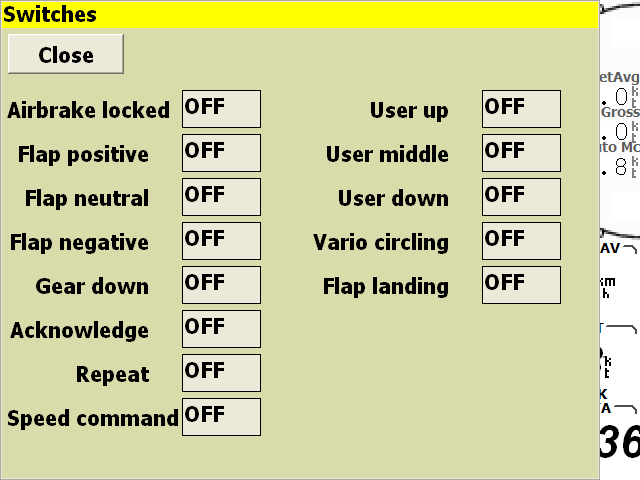
\includegraphics[angle=0,width=0.7\linewidth,keepaspectratio='true']{figures/dialog-switches.png}
\end{center}

\section{Modo escravo}

O tipo de ajuste de dispositivo nas configurações “NMEA out” pode ser definida para o uso de dois Altair ou sistemas PDA em modo mestre-escravo.  O modo mestre, o segundo dispositivo de comunicação pode ser ajustado para NMEA Out e todos os dados recebidos da primeira porta de comunicação do dispositivo (bem como dados exportados) serão enviados ao escravo.

Como um exemplo onde dois Altairs estão conectados entre si, no escravo, o primeiro dispositivo pode ser ajustado para “VEGA” ou “Altair Pro” e este sistema recebe todos os dados e se torna o GPS mestre e conectado aos instrumentos (Vega, FLARM, etc.).


\section{Estado do sistema}\label{sec:system-status}

Usada primariamente como um verificador do sistema, para ver como o computador e os dispositivos conectados estão funcionando.  É acessado através do menu e selecionada a aba {\bf Sistema}.
\sketch{figures/status-system.png}

Todos os valores dinâmicos (voltagem da bateria, números de satélites capturados) são atualizados continuamente.  

\section{Dispositivos múltiplos }

Você pode configurar até dois dispositivos externos, conectados ao mesmo tempo (alguns PDAs têm duas portas seriais, mas o bluetooth pode gerenciar qualquer número de conexões simultâneas).

Quando ambos fornecem um dado de GPS válido, o primeiro é escolhido pelo XCSoar e o segundo dado de GPS é ignorado.  Se o primeiro dispositivo falhar, o XCSoar alterna para o segundo automaticamente, até que o primeiro se recupere.

O mesmo é válido para todos os valores (altitude barométrica, variômetro, velocidade do ar, tráfego, ....) e o XCSoar dará preferência para o primeiro dispositivo e usa o segundo somente para valores que não foram recebidos pelo primeiro dispositivo.

Exemplo: o primeiro dispositivo é um CAI 302 e o segundo é o FLARM.  Assim fornece o melhor dos dois: o XCSoar tem a velocidade do ar, variômetro e dados de tráfego.  



\section{Gerenciando dispositivos externos}

A janela de gerenciamento de dispositivos pode ser acessada através do menu de configuração.
\menulabel{\bmenug{Config 2}\blink\bmenug{Dispositivos}}. Mostra uma lista de dispositivos externos configurados e quais informações são mostradas.

\config{comdevices}
O botão “Reconectar” tentar reconectar os dispositivos selecionados.  O XCSoar reconecta periodicamente os dispositivos com falha, mas algumas veze pode ser necessário conectar manualmente.

O botão “Baixar vôo” só estará disponível com registradores IGC (veja a lista na seção \ref{sec:supported-varios}).  Clicando no item, o XCSoar mostra a lista de vôo e pergunta qual selecionar.  O arquivo IGC pode ser baixado da pasta “LOGS” no diretório \texttt{XCSoarData}.

O botão “GERENCIAR” é ativo quando há conexão com o Vega ou CAI 302.  Fornece acesso às funções especiais destes dispositivos, como limpar a memória de vôo do CAI 3022, que algumas vezes é necessária para se resolver uma falha de firmware.  
